\documentclass[conference]{IEEEtran}
\IEEEoverridecommandlockouts

\usepackage{cite}
\usepackage{amsmath,amssymb,amsfonts}
\usepackage{graphicx}
\usepackage{textcomp}
\usepackage[official]{eurosym}
\usepackage{xcolor}
\usepackage{booktabs}
\usepackage{siunitx}
\usepackage{url}
\usepackage{hyperref}
\hypersetup{colorlinks=true,linkcolor=blue,citecolor=blue,urlcolor=blue}

\def\BibTeX{{\rm B\kern-.05em{\sc i\kern-.025em b}\kern-.08em
    T\kern-.1667em\lower.7ex\hbox{E}\kern-.125emX}}

\begin{document}

\title{Solder-Paste Printing and Die-Bonder Placement of Micro-LEDs:\\
Capillary Self-Alignment and Die Tilt\\
{\normalsize Course report — ET4277 + ET4391 — Part 2}}

\author{\IEEEauthorblockN{Daniel Tyukov}
\IEEEauthorblockA{\textit{Department of Microelectronics, ECTM + ITEC}\\
\textit{Delft University of Technology}\\
Delft, the Netherlands \\
Student no. 5714699 \;\textbar\; \texttt{daniel.tyukov@alphait.us}}
}

\maketitle

\begin{figure}[!t]
  \centering
  
\includegraphics[width=0.3\columnwidth]{figures/tudelft_logo.pdf}
\end{figure}

\begin{abstract}
Part 1 described the test board. This part documents the die-bonding
process used to populate it with micro-LEDs and analyses the physics that
governs the result. After completing the EKL safety training and gaining
access to the cleanroom measurement lab, I attended a bonding session run
by Ahmed Abdelwahab, who placed W\"urth WL-SFCC 0404 RGB LEDs on the
existing v1 board and trained me on the workflow. The v2 board from Part 1
was still in fabrication, so the session used the v1 board, which carries
the same LED footprint. The process is deliberately low-tech: solder paste
is printed by hand through a
100~$\mu$m stencil, the dies are placed with a Tresky die bonder, and the
joint forms on a hot plate. The physics worth studying is in the last step.
When the Sn42/Bi57.6/Ag0.4 paste melts, surface tension pulls each die
toward the centre of its pad set, which is convenient, but the same forces
can tilt a die and lock it in a crooked position that never recovers. The
contribution of this report is on the analysis side: it documents the
printing and placement steps, then reads the self-alignment and tilt
behaviour against the capillary self-alignment literature to identify which
process variable matters most. That variable is solder volume. Manual
stencil printing gives no volume metering, and volume is exactly the
quantity the literature ties most strongly to both placement accuracy and
the non-restoring tilt mode.
\end{abstract}

\begin{IEEEkeywords}
micro-LED, die bonding, solder paste, stencil printing, capillary
self-alignment, die tilt, reflow, cleanroom
\end{IEEEkeywords}

\section{Introduction}

The bond joint under a micro-LED is the part of the device that the
electrical tests in Part 1 were built to characterize. Before any of those
measurements can run, the LEDs have to be on the board, and how they get
there decides what the joint looks like. This part documents that step and
analyses why it behaves the way it does.

The plan with Ahmed was straightforward. Part 1 was the design mini-project.
For Part 2, since I am taking ET4277 and ET4391 together, we agreed that he
would assemble LEDs on the die bonder while I documented the workflow and
wrote a literature-based analysis of self-alignment and die
tilt~\cite{abdelwahab2025ectc}. The one hard constraint on the board came
out of this: it has to fit the die-bonder chuck, so the outline was kept at
9.3~cm $\times$ 9.3~cm, inside the 9.5~cm limit.

Solder bonding is attractive for micro-LEDs because it does three things at
once: it mechanically fixes the die, it makes the electrical contact, and,
if the geometry is right, it pulls the die into alignment on its own as the
solder melts~\cite{mastrangeli2017csa}. That last effect, capillary
self-alignment, is the reason this is worth studying rather than just
doing. It can reach micron-level accuracy with no extra
equipment~\cite{vareilles2024solder}, but it is not free of failure modes,
and the dominant one for small dies is tilt~\cite{berthier2015tilt}.

\section{Background: How Micro-LEDs Get onto a Substrate}

A micro-LED is a GaN die between roughly 1 and 100~$\mu$m on a side, grown on
a donor wafer and then moved onto a display or test substrate where it has
to be both mechanically held and electrically
contacted~\cite{li2020masstransfer}. Moving millions of them is the step the
field calls mass transfer, and it is the recognized bottleneck for micro-LED
commercialization~\cite{li2020masstransfer}. The methods split into two
families, and it helps to place where the bonding done in this work sits.

\textbf{Pick-and-place and its variants.} Fine pick-and-place, roll
printing, and laser-assisted transfer move dies deterministically, one or a
batch at a time. They are accurate but serial, and the placement machine's
own accuracy becomes the limit as the die
shrinks~\cite{ji2022selfassembly}. The die-bonder flow in this report is the
prototyping-scale version of this family: a machine picks each die and sets
it on a pad.

\textbf{Self-assembly.} The alternative lets the dies place themselves in
parallel under a field, gravity, or, most relevant here, the capillary force
of a molten alloy~\cite{ji2022selfassembly}. Cho et al.\ pushed this to an
extreme, assembling 19{,}663 GaN micro-LEDs of 45~$\mu$m diameter at 99.9\%
yield in under a minute by shaking them over a substrate patterned with
molten low-melting-point alloy on gold pads, where the capillary force of
the wetting alloy pulls each die onto its site~\cite{cho2019fsa}. The
throughput is enormous because no machine places the dies.

The two families share the physics this report is about. Even in
deterministic placement, once the solder melts the capillary force corrects
the position, so the machine only has to get the die close; self-assembly
takes that same force and makes it do the whole job. Either way the molten
joint aligns the die, and either way the failure mode is the same: the die
can tilt rather than settle flat. Studying self-alignment and tilt on a
die-bonder-placed LED is therefore directly informative for where the field
is heading. The gold (ENIG) pads of the board matter here too, since wetting
of the molten alloy to gold is what generates the aligning
force~\cite{cho2019fsa}.

\section{Cleanroom Access and Training}

Access to the EKL cleanroom needed two things first. I completed the EKL
safety training and was granted access to the cleanroom and its measurement
lab. Ahmed then ran a die-bonding session and trained me on the full flow:
how the stencil and paste are handled, how the Tresky die bonder is set up
and jogged, how the dies are picked and placed, and how the board is
reflowed. The session used Ahmed's existing v1 board (panel E1664138) from
the ECTC 2025 work~\cite{abdelwahab2025ectc}, not the v2 board from Part 1,
which was still in fabrication at the time. The v1 board carries the same
W\"urth WL-SFCC 0404 footprint, so the process and the pad geometry
transfer directly to the v2 board once it arrives. The figures in this
report are from that session; the analysis that follows is my own, built
from the workflow and the self-alignment literature.

\section{Printing and Placement}

\begin{figure}[!t]
  \centering
  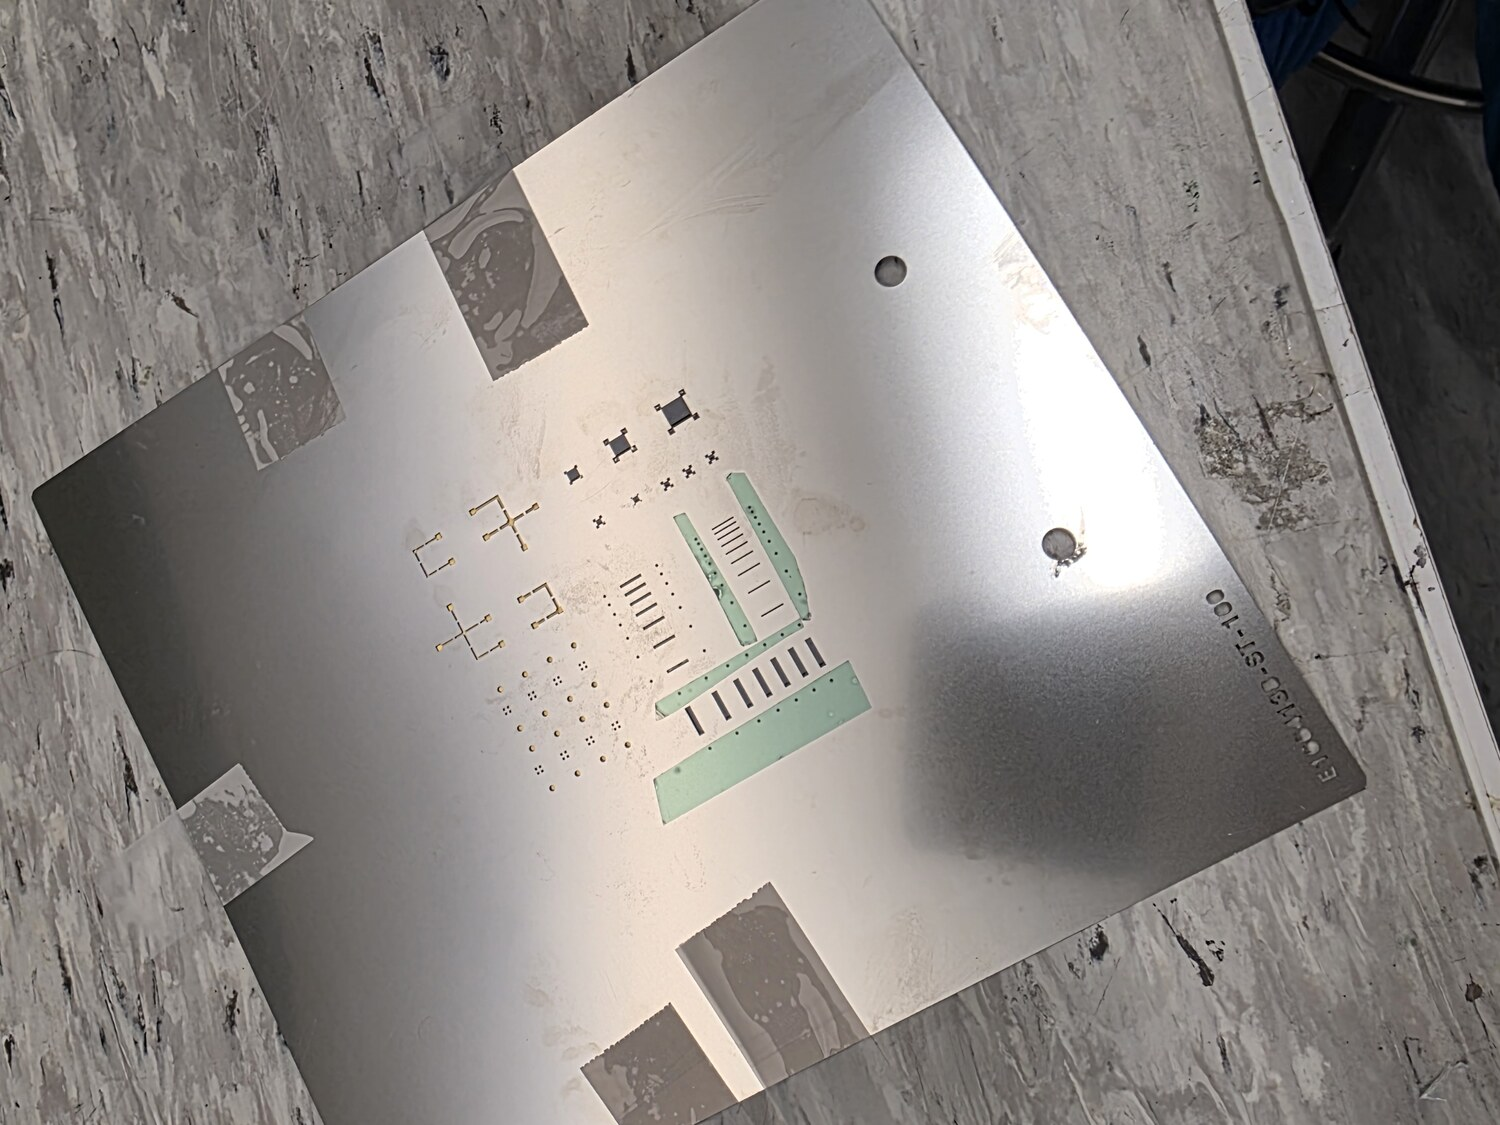
\includegraphics[width=0.9\columnwidth]{figures/stencil_setup.jpg}
  \caption{Manual stencil printing. The 100~$\mu$m laser-cut stainless
  stencil is taped flat over the PCB with green polyimide tape; paste is
  pushed across the apertures with a plastic spatula and the excess scraped
  back with a razor blade.}
  \label{fig:stencil}
\end{figure}

\subsection{Stencil printing}

The deposition is manual. The tools are a roll of green polyimide tape, the
PCB, a 100~$\mu$m laser-cut stainless-steel stencil (the same eC-stencil-mate
type Eurocircuits ships with their boards), a plastic spatula, and a razor
blade (Fig.~\ref{fig:stencil}). The stencil is aligned over the board and
taped down flat, paste is dragged across the apertures with the spatula,
and the blade scrapes the excess back. Lifting the stencil leaves a paste
deposit on each LED pad.

The paste is Chip Quik TS391LT, a thermally stable no-clean
Sn42/Bi57.6/Ag0.4 alloy, T4 mesh (20--38~$\mu$m particles), 87\% metal by
weight, with a 138~$^\circ$C melting point~\cite{chipquik_ts391lt}. The low
melting point is the point: a bismuth alloy reflows around
138--165~$^\circ$C instead of the 217~$^\circ$C+ of SAC305, which keeps the
thermal load on the die low.

This method has real advantages. It needs no equipment, it is fast, it is
portable, and it works directly with the Eurocircuits stencils and boards.
The catch is that the deposit is whatever the operator and the stencil give
you: there is no volume metering, the reproducibility is medium, and the
smallest aperture that printed cleanly was 0.4~$\times$~0.4~mm$^2$, right at
the LED pad size. Fig.~\ref{fig:array} shows printed deposits across the
LED array, and Fig.~\ref{fig:paste} is a single site under the die-bonder
camera. The deposits are usable but visibly uneven from pad to pad.

\begin{figure}[!t]
  \centering
  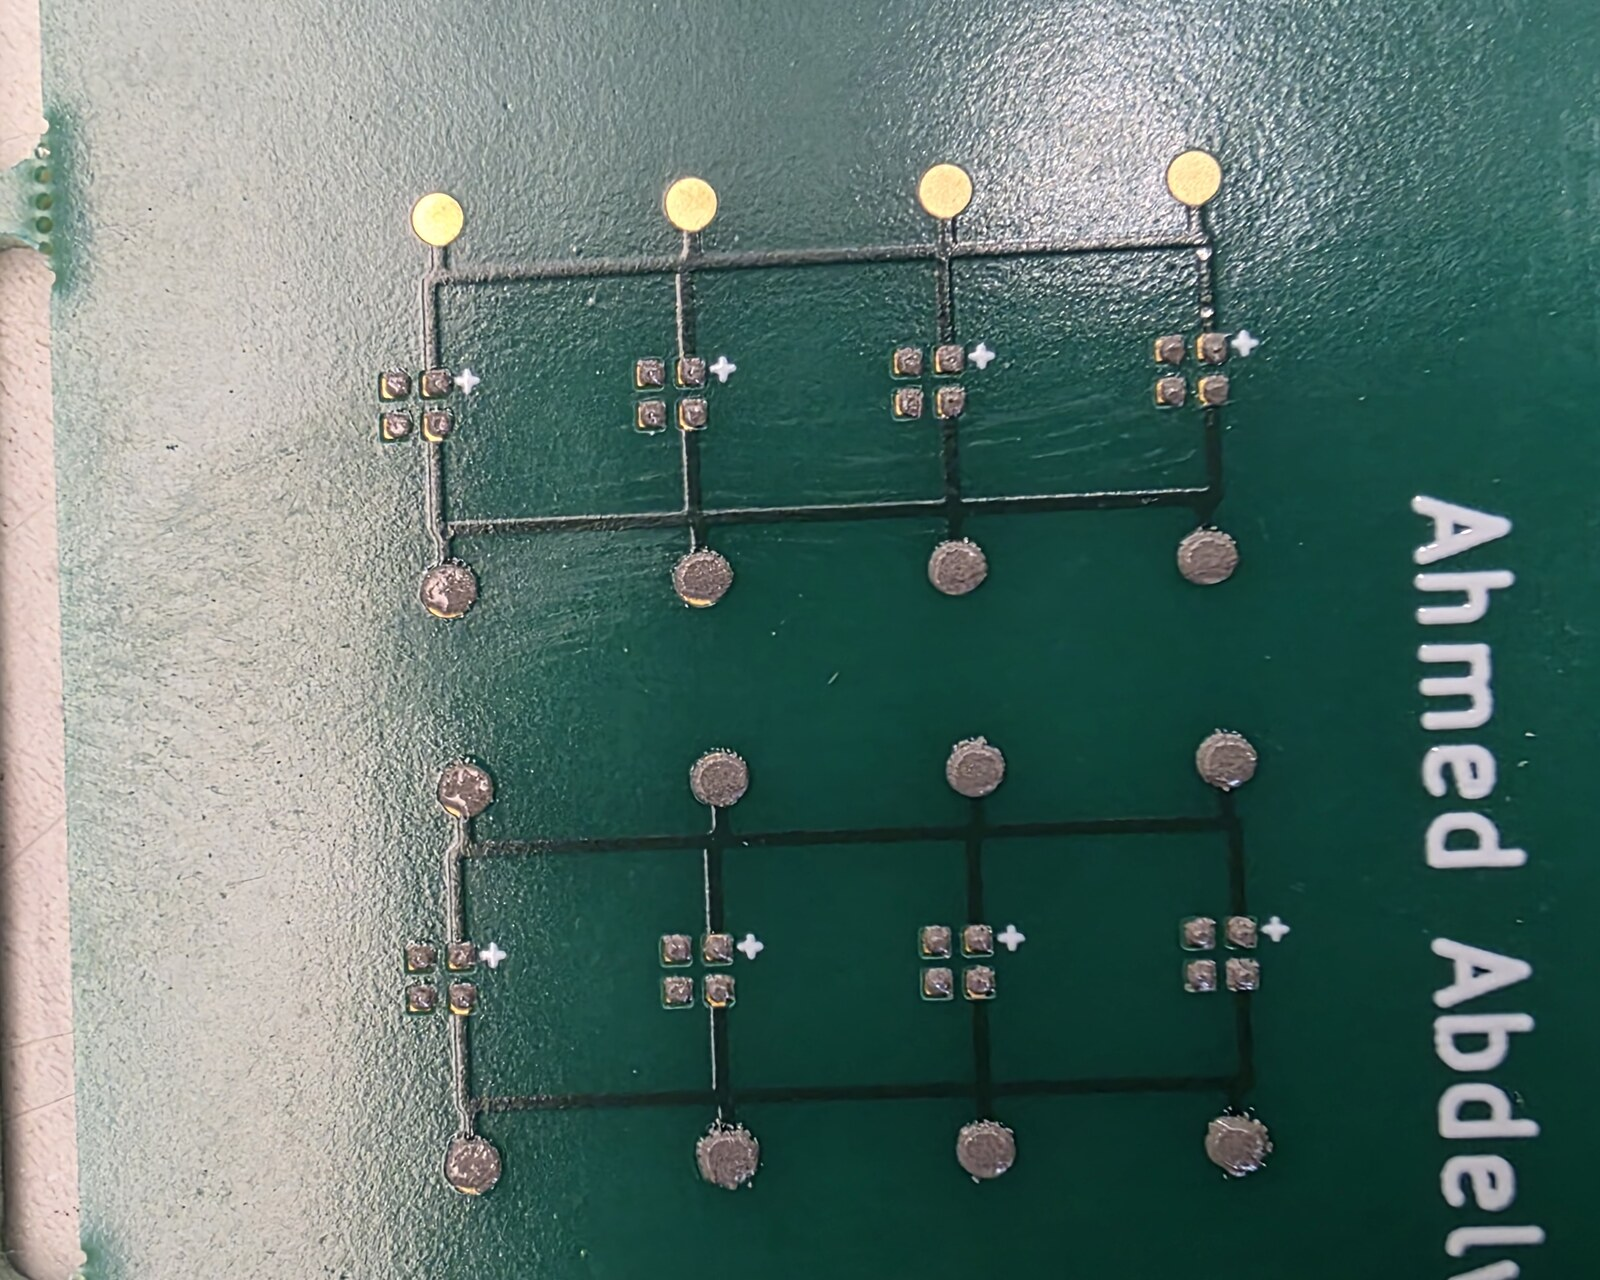
\includegraphics[width=0.9\columnwidth]{figures/printed_array.jpg}
  \caption{LED footprints after printing, board still in its Eurocircuits
  panel. Each four-pad site carries a small paste deposit; deposit size and
  shape vary noticeably between sites, which is the main limitation of
  hand printing.}
  \label{fig:array}
\end{figure}

\subsection{Die placement}

\begin{figure}[!t]
  \centering
  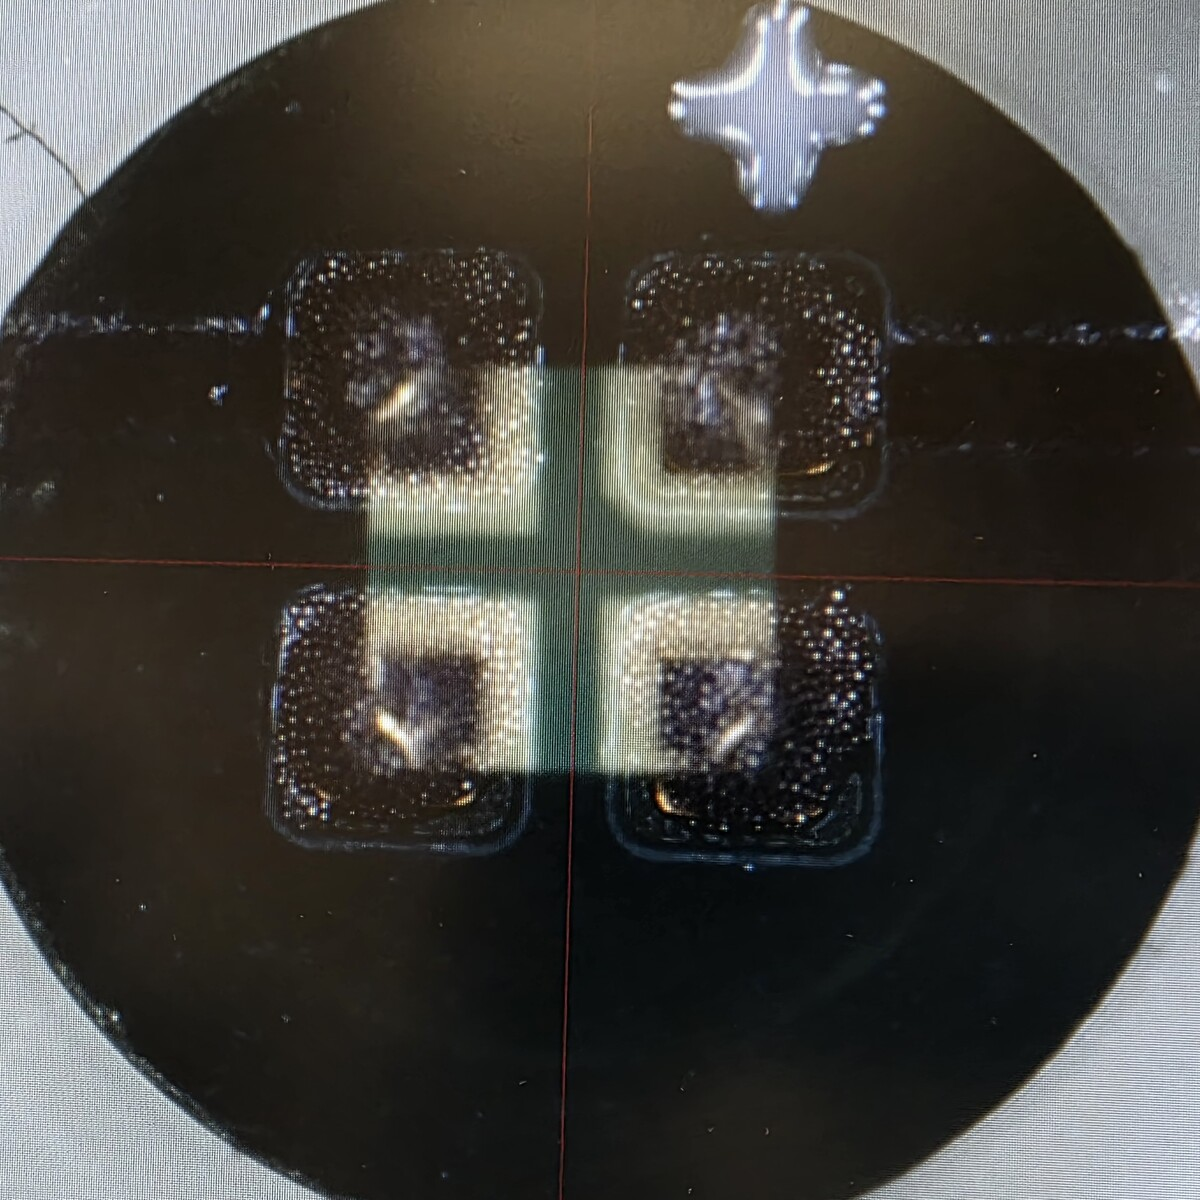
\includegraphics[width=0.78\columnwidth]{figures/paste_highmag.jpg}
  \caption{One LED footprint at high magnification through the die-bonder
  camera. The four 0.4~mm pads each hold a grainy paste deposit; the cross
  is a placement fiducial. The dark cross between the pads is the
  soldermask web that separates the anode and the three cathodes.}
  \label{fig:paste}
\end{figure}

Placement runs on a Tresky die bonder (Fig.~\ref{fig:bonder}). The board
sits on the heated vacuum chuck and the dies wait in a ceramic tray. The
machine picks a die, the camera lines it up against the pad fiducial, and
it sets the die down on the paste. The placement parameters used were a
100~g place force, a 20~ms place time, and a 40~ms blow-off. These are
gentle numbers, which is what you want: the paste has to hold the die by
tack until reflow, and pressing too hard squeezes paste out from under the
die and starves the joint.

Placement accuracy by hand-jogged die bonder is only moderate.
Fig.~\ref{fig:placed} shows a die just after it was set down: it sits low
and slightly rotated relative to the crosshair that marks the pad centre.
This offset is normal and, within limits, fine, because the next step is
supposed to correct it.

\subsection{Paste and reflow}

The choice of paste shapes the whole alignment step, because the die only
moves while the solder is liquid. The TS391LT is a near-eutectic
Sn42/Bi57.6/Ag0.4 alloy with a 138~$^\circ$C melting point, well below the
217~$^\circ$C of SAC305. For a GaN micro-LED this low budget matters: less
heat into the die means less thermal stress on the epitaxy and on the
nascent joint. The trade-off is that bismuth alloys are more brittle than
SAC, so the joint is mechanically weaker, which is acceptable here because
the boards are for characterization rather than field service.

Reflow was done on a hot plate toward a peak near 165~$^\circ$C. The window
between melting at 138~$^\circ$C and the peak is the time the joint is
liquid and therefore the time available for self-alignment to act. This is
the part of the process least under control in a manual flow: a hot plate
heats from the bottom and the board's thermal mass and contact set the real
profile, so the liquidus time varies between runs. Since the capillary
restoring motion needs a finite time to bring the die home before the
solder freezes, an inconsistent profile turns directly into inconsistent
alignment, on top of the volume variation from hand printing.

\begin{figure}[!t]
  \centering
  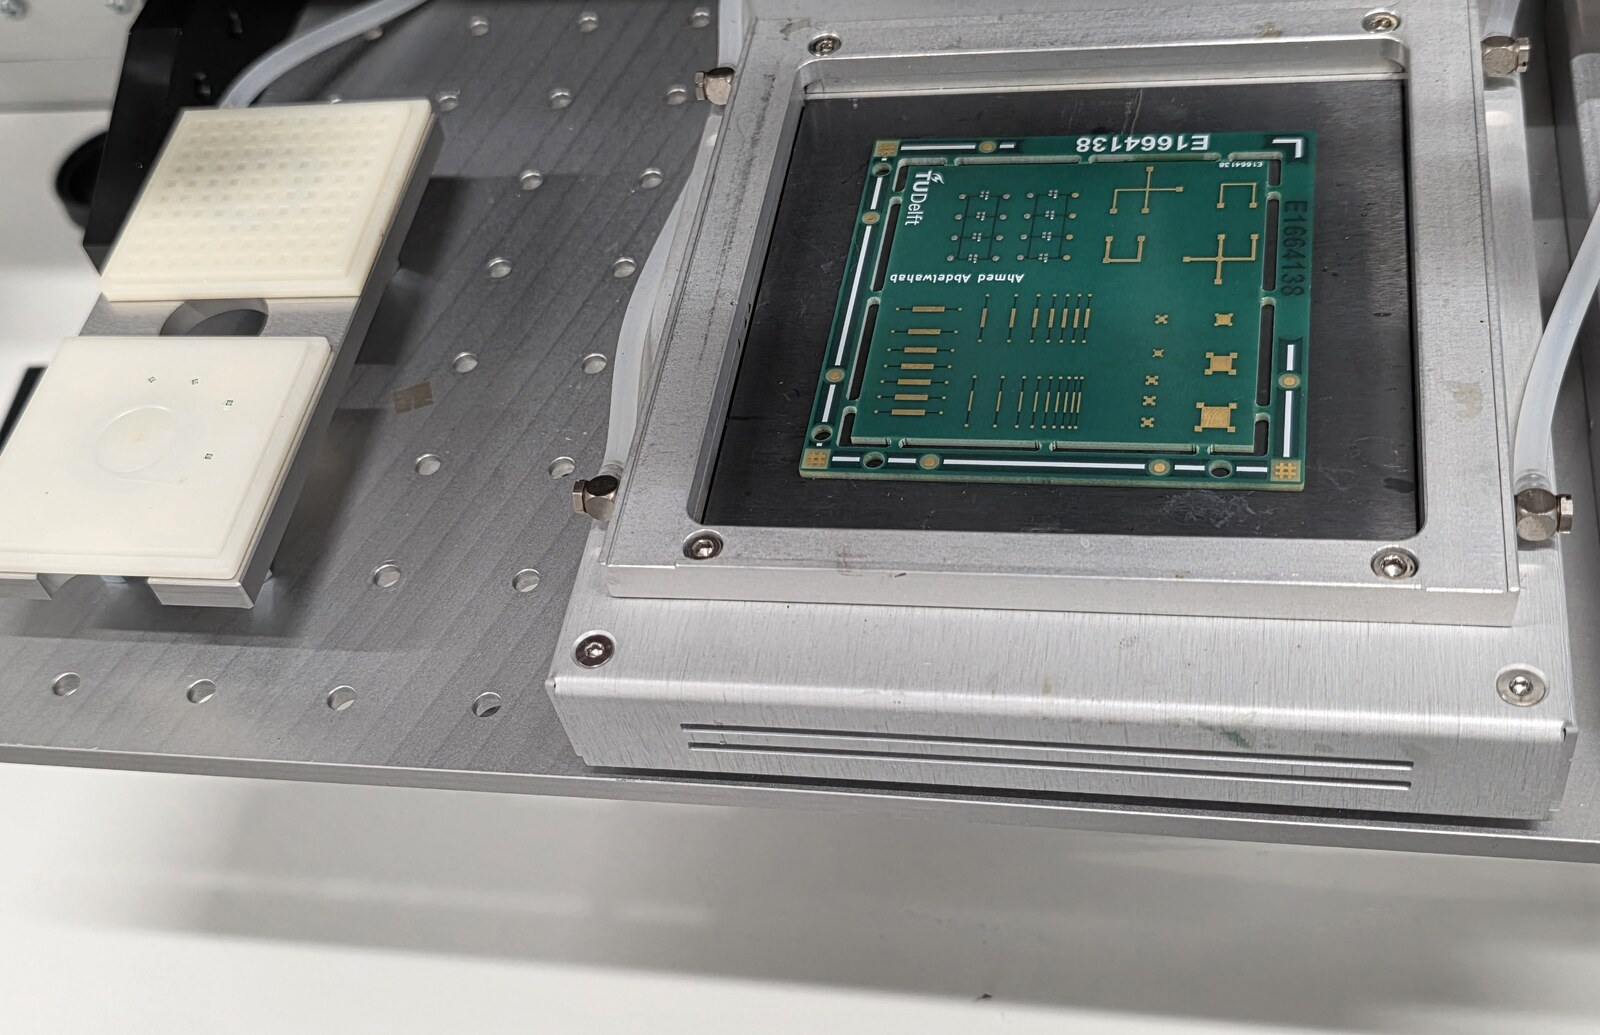
\includegraphics[width=0.95\columnwidth]{figures/board_bonder.jpg}
  \caption{The board mounted on the Tresky die bonder's heated chuck, with
  the LED dies in the white ceramic tray at left. The optical breadboard
  underneath isolates the placement head from vibration.}
  \label{fig:bonder}
\end{figure}

\section{Self-Alignment and Die Tilt}

\subsection{Why the die moves on its own}

When the paste melts, the joint becomes a liquid bridge between the die and
its pads. Surface tension tries to minimize the surface energy of that
bridge, which means it pulls the die toward the position where the molten
solder columns are shortest and most symmetric, i.e.\ centred on the
pads~\cite{mastrangeli2015fluidjoint, mastrangeli2017csa}. For a molten
solder the surface tension is around 500~mN/m and the capillary length is
about 2~mm~\cite{mastrangeli2015fluidjoint}, so for a sub-millimetre die
the capillary force easily dominates gravity. The restoring force scales
with the in-plane offset, so a die placed slightly off-centre
(Fig.~\ref{fig:placed}) gets dragged back during reflow. This is the
mechanism that makes the moderate placement accuracy acceptable.

How much offset the joint can absorb is not small. Krammer et al.\ modelled
the chip during reflow with four forces — surface tension, hydrostatic and
capillary pressure, gravity, and dynamic friction — and showed by
experiment that surface tension dominates the in-plane
motion~\cite{krammer2007reflow}. In their measurements, surface-mount chips
self-aligned even from initial misplacements of
400--500~$\mu$m~\cite{krammer2007reflow}, with average correction distances
around 249~$\mu$m along one axis~\cite{krammer2008movement}. They also found
the alignment is anisotropic and geometry-dependent: parts with metallized
sidewalls (so the solder can wet a vertical face) self-align noticeably
better than parts without~\cite{krammer2008movement}. That is encouraging
for the WL-SFCC, whose four bottom contacts give the molten joint defined
features to pull against, and it sets a generous tolerance budget against
the moderate die-bonder placement of Fig.~\ref{fig:placed}.

The recent work of Lesueur et al.\ puts numbers on the accuracy ceiling.
Using mass reflow of corner solder pillars they reached lateral alignment
better than 2~$\mu$m, and in some configurations under 1~$\mu$m, with
measured z-tilt variation also below 1~$\mu$m, and they showed this
self-alignment absorbs standard flip-chip pick-and-place placement
tolerances outright~\cite{lesueur2025selfalign}. The lesson for the manual
process here is that the achievable accuracy is set by the joint geometry
and the solder, not by how carefully the die is placed.

\begin{figure}[!t]
  \centering
  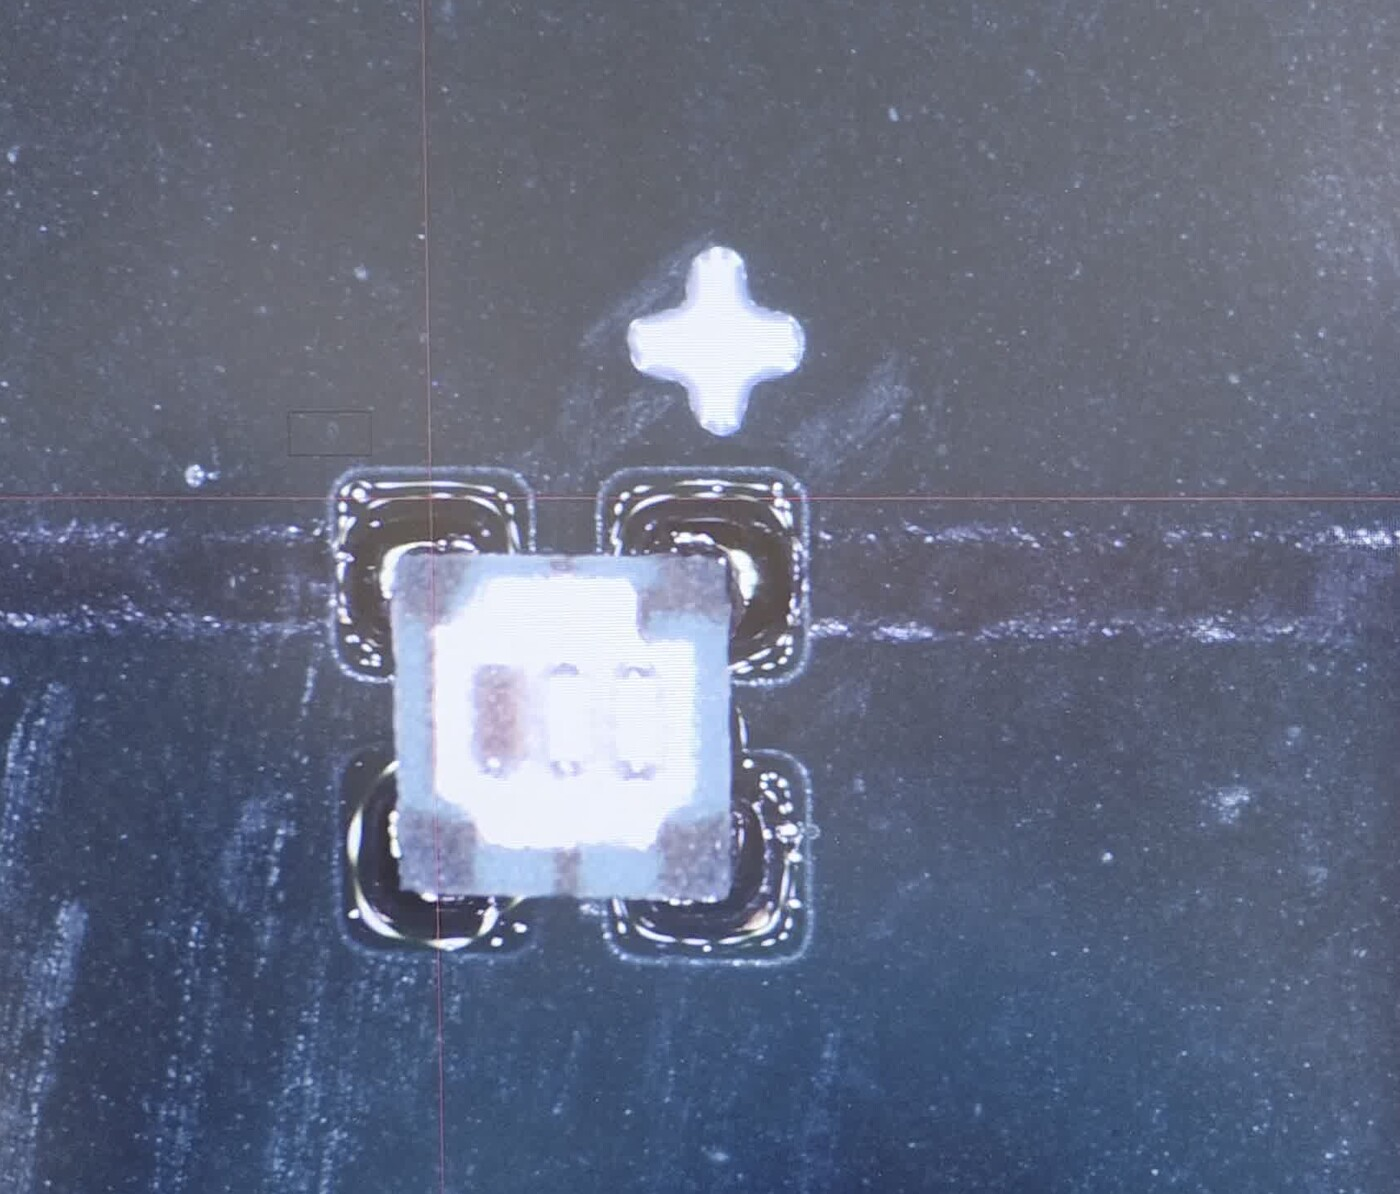
\includegraphics[width=0.95\columnwidth]{figures/die_placed.jpg}
  \caption{A WL-SFCC die set down on the printed paste, seen through the
  die-bonder camera. The die straddles the four pads but sits offset and
  rotated relative to the crosshair (pad centre) and the cross fiducial
  above it. Capillary forces are expected to pull this offset out during
  reflow; the risk is that the same forces tilt the die instead.}
  \label{fig:placed}
\end{figure}

\subsection{The tilt problem}

A floating die has four ways to move: shift, twist, lift, and tilt. Three
of them are stable, meaning the capillary force restores the die toward
alignment if it is perturbed. Tilt is the exception: it is
non-restoring~\cite{berthier2015tilt}. Once a die starts to rock, the
solder geometry does not push it flat again, and for a small die with a
thin solder layer the low corner can touch the pad and pin the die in a
tilted position that reflow never undoes. Berthier et al.\ show exactly
this with an LED on solder, and note that avoiding it otherwise requires
near-perfect horizontality at drop-off, which is hard to guarantee on a
hand-jogged machine~\cite{berthier2015tilt}. The older reflow-dynamics
models capture why: the Ellis-Masada picture has the chip rotate about a
corner that stays pinned to the pad~\cite{krammer2008movement}, so any
asymmetry in the solder under the four corners feeds straight into a tilt
the joint cannot correct.

The variable that couples placement, alignment, and tilt is the solder
volume. Vareilles et al.\ measured this directly for sub-millimetre cells
and found the best placement accuracy with low solder volume, a receptor
pad smaller than the die, and an initial offset of about 10\% of the die
size; too much solder both shifts and tilts the part~\cite{vareilles2024solder}.
That is the uncomfortable conclusion for the process I ran: hand stencil
printing has no volume control, and volume is the one knob that matters
most. The uneven deposits in Figs.~\ref{fig:array} and~\ref{fig:paste} are
the visible form of that problem.

\section{Analysis and Suggestions}

Reading the process against the literature, and discussing it with Ahmed,
points to four conclusions:

\textbf{The print is the weak link, not the placement.} The die bonder
places to moderate accuracy and the capillary force forgives the rest, so
chasing tighter placement is not where the effort should go. The deposit
volume and its pad-to-pad consistency are what set how well, and how flat,
each die ends up. A finer or volume-controlled deposition (a thinner
stencil for these pads, or jetting the paste) would attack the actual
limiting variable.

\textbf{Keep the solder volume low and the pad inside the die footprint.}
Following Vareilles et al., a pad slightly smaller than the die and a
modest deposit should give a stronger, flatter pull than a generous
deposit on a matched pad~\cite{vareilles2024solder}. The current 0.4~mm
pads sit right at the die contact size, so there is room to trim them.

\textbf{Tilt is the failure to watch, not shift.} Because shift and twist
self-correct and tilt does not, inspection should look for rocked dies
specifically, ideally in cross-section or with side-view imaging rather
than top-down, which hides tilt. If tilt turns out to be common, the
lyophilic-band trick from Berthier et al.\ — patterning the wettable area
to constrain the liquid and stabilize the tilt mode — is the
design-side fix~\cite{berthier2015tilt}, and it would go straight onto a
future revision of the board.

\textbf{Mind the reflow profile.} The TS391LT melts at 138~$^\circ$C and we
reflowed on a hot plate toward a peak near 165~$^\circ$C. Hot-plate reflow
heats from the bottom and the temperature is not as controlled as an oven
profile, so the time the joint spends liquid, which is the time available
for self-alignment, varies. A logged profile would make the alignment
window repeatable.

\begin{figure}[!t]
  \centering
  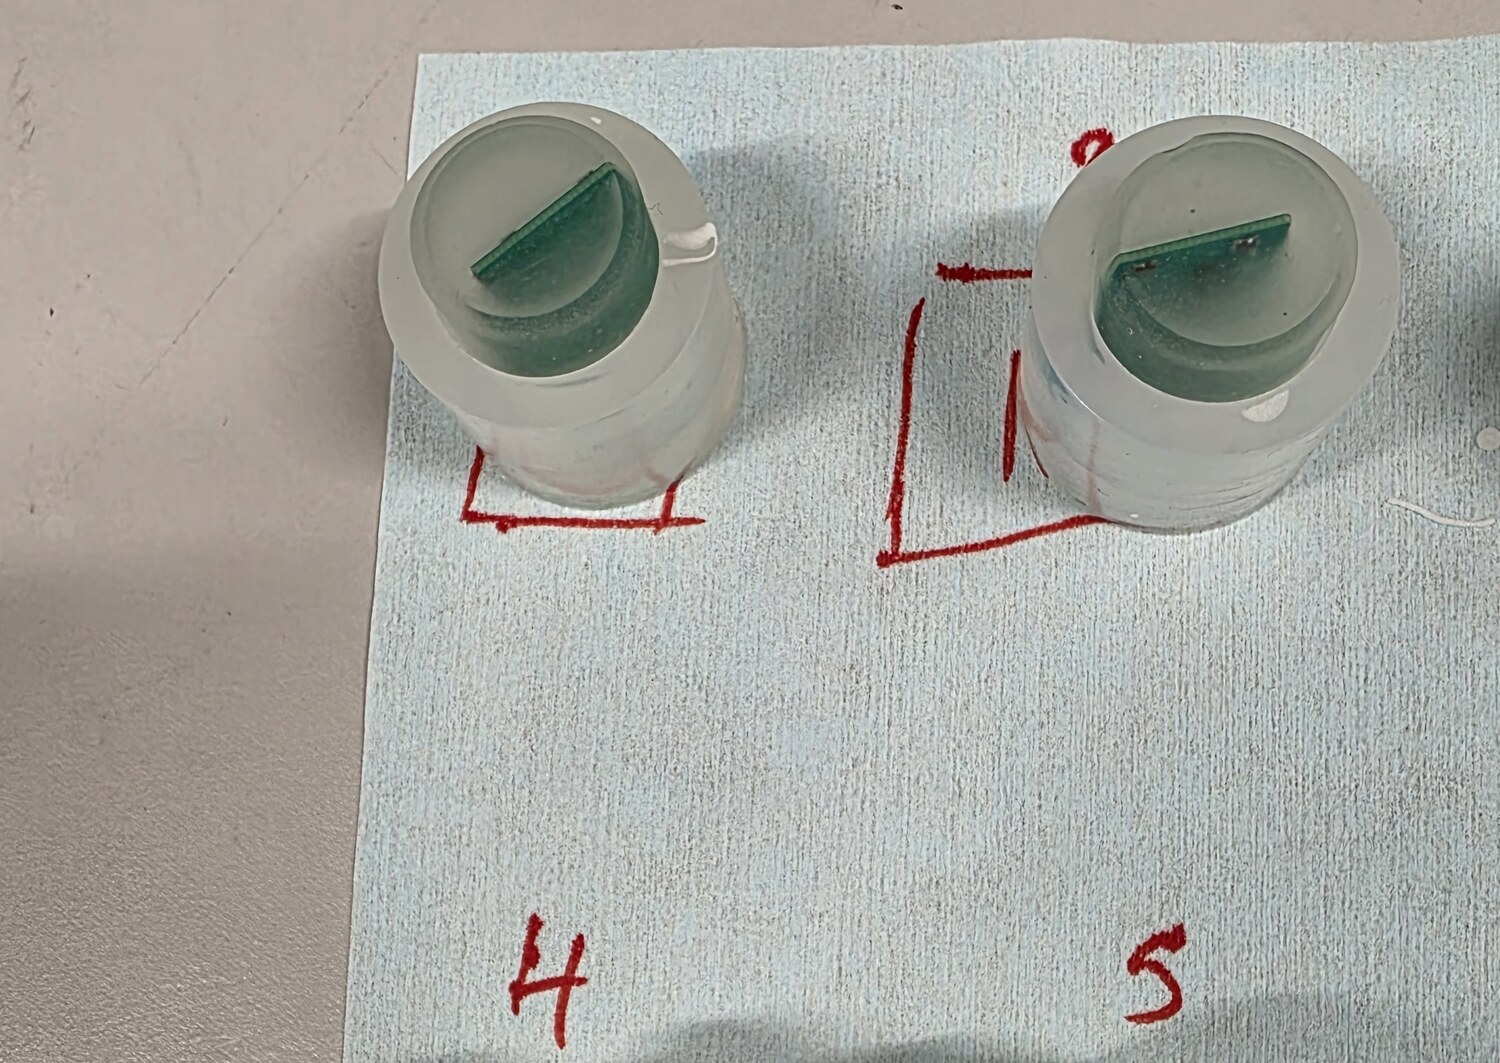
\includegraphics[width=0.85\columnwidth]{figures/samples.jpg}
  \caption{Diced board coupons with bonded LEDs, sealed in labelled vials
  after the session. Cutting the board into per-site coupons lets each
  bonded LED be cross-sectioned or imaged from the side, which is the view
  that actually reveals tilt.}
  \label{fig:samples}
\end{figure}

\section{Conclusion}

WL-SFCC micro-LEDs were bonded in the EKL cleanroom in a session run by
Ahmed, which I attended after completing the EKL safety training, gaining
cleanroom and measurement-lab access, and being trained on the die-bonding
flow. The process — hand stencil printing of a low-melting Sn/Bi/Ag paste,
die-bonder placement, hot-plate reflow — is cheap and fast, and the
capillary self-alignment of the molten joint covers the moderate placement
accuracy. The analysis here identifies solder-volume control as the
limiting variable: the literature ties volume to both alignment accuracy
and the non-restoring tilt mode, and hand printing does not control it. The
concrete next steps that follow from this are tighter deposit control, pads
trimmed inside the die footprint, tilt-aware inspection, and a logged
reflow profile. The session was run on the v1 board; once the v2 boards
from Part 1 arrive from the fab, the same process and these same
conclusions apply directly, and the bonded v2 boards are what the
electrical characterization will run on. The samples from this session were
diced and stored for inspection (Fig.~\ref{fig:samples}); side-view imaging
of those coupons is the natural next check, since it is the one view that
shows tilt directly rather than hiding it.

\section*{Acknowledgment}

I thank Ahmed Abdelwahab for the cleanroom training and for the
discussions on self-alignment and tilt that shaped this report.

\bibliographystyle{IEEEtran}
\bibliography{refs}

\end{document}
